
\usetikzlibrary{shadows,arrows}
\usetikzlibrary{decorations.markings}

% Define the layers to draw the diagram
\pgfdeclarelayer{background}
\pgfdeclarelayer{foreground}
\pgfsetlayers{background,main,foreground}

% Define block styles  
\tikzstyle{blockstyle}=[draw, fill=blue!20, text width=6.0em, text centered,
  minimum height=1.5em,drop shadow]
\tikzstyle{textbox} = [blockstyle, text width=8em, minimum width=10em,
  minimum height=3em, rounded corners, drop shadow]

\tikzstyle{texto} = [above, text width=6em, text centered]

\tikzset{
    big arrow/.style={
        decoration={markings,mark=at position 1 with {\arrow[scale=2,#1]{>}}},
        postaction={decorate},
        shorten >=0.4pt}}

\tikzstyle{line} = [draw, thick, color=black!50, big arrow]
% Define distances for bordering

\newcommand{\class}[2]{node (p#1) [textbox] {#2}}
 
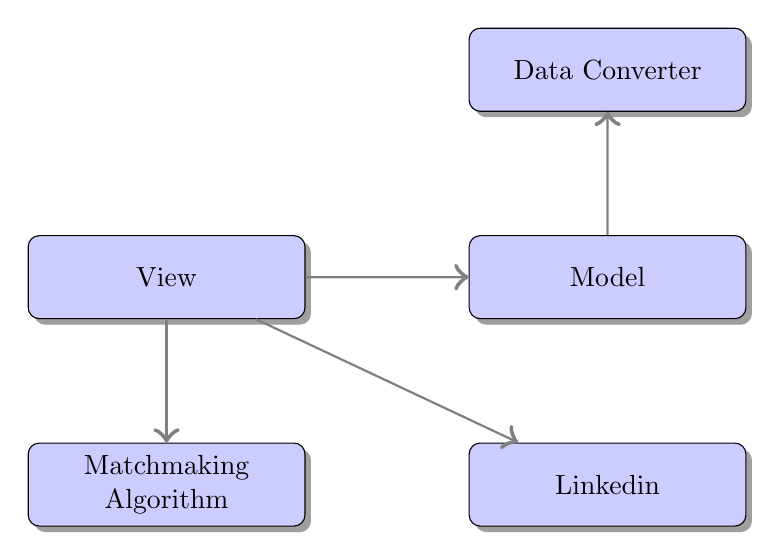
\begin{tikzpicture}[scale = 0.7]
% Draw diagram elements
\path                         \class{1}{View};
\path (p1.south) +( 0.0,-3.0) \class{2}{Matchmaking Algorithm};
\path (p1.south) +( 8.0,-3.0) \class{3}{Linkedin};
\path (p3.north) +( 0.0, 3.0) \class{4}{Model};
\path (p4.north) +( 0.0, 3.0) \class{5}{Data Converter};

% Draw arrows between elements
\path [line] (p1) -- node [left] {} (p2);
\path [line] (p1) -- node [left] {} (p3);
\path [line] (p1) -- node [left] {} (p4);
\path [line] (p4) -- node [left] {} (p5);
\end{tikzpicture}


